% Sección generada a mano; cifras por macros (tablas/macros.tex).
Para probar la generalidad entre datasets agregamos dos benchmarks reales ampliamente usados, con la serie
como unidad estadística: SMD (\Nu{smd} máquinas) y SMAP+MSL (\Nu{nasa} canales; el canal P-2 aparece dos
veces en el archivo de etiquetas original y se cuenta una vez). La Tabla~\ref{tab:bench} resume los
resultados. \textbf{Aquí las mejoras no generalizan como en los bloques anteriores}, y lo reportamos tal cual.

\paragraph{SMD.} El método final queda por debajo del artículo en AUPRC (\Hy{smd}{H1}{mean}
\Hy{smd}{H1}{ci}, gana en \Hy{smd}{H1}{wins} de \Hy{smd}{H1}{n} máquinas; $p_{\text{Holm}}=$ \Hy{smd}{H1}{ph},
no significativo tras la corrección) y en AUROC (\Me{smd}{art}{auroc} $\to$ \Me{smd}{fin}{auroc}). El diseño
factorial identifica la causa: es la proyección. \MIII{} sola pierde frente al artículo en
\Hy{smd}{H5a}{losses} de \Hy{smd}{H5a}{n} máquinas (H5a: \Hy{smd}{H5a}{mean} de AUROC, $p_{\text{Holm}}$
\Hy{smd}{H5a}{ph}; H5b: \Hy{smd}{H5b}{mean} de AUPRC), mientras que el recorte con umbral IQR sin \MIII{}
(\MI+\MII{}) obtiene el mejor AUPRC del bloque (\Me{smd}{m1m2}{auprc} frente a \Me{smd}{art}{auprc}).
Isolation Forest (\Me{smd}{ifo}{auroc} de AUROC) iguala al método final y queda por debajo del artículo.

\paragraph{SMAP+MSL.} Las diferencias son pequeñas. El método final empata con el artículo en AUPRC
(H1: \Hy{nasa}{H1}{mean} \Hy{nasa}{H1}{ci}) y lo supera ligeramente en AUROC (\Me{nasa}{art}{auroc} $\to$
\Me{nasa}{fin}{auroc}); aquí el recorte sí aporta (H3a: \Hy{nasa}{H3a}{mean}, $p_{\text{Holm}}$
\Hy{nasa}{H3a}{ph}; \MII{} sola: AUROC \Me{nasa}{m2}{auroc}), y \MIII{} sola pierde un poco en AUPRC
(H5b: \Hy{nasa}{H5b}{mean}). El mejor método del bloque es Isolation Forest (AUROC \Me{nasa}{ifo}{auroc}); en
este benchmark ninguna variante basada en TracIn está lejos del azar (AUROC $\approx 0.6$).

\paragraph{Por qué \MIII{} no ayuda en estos benchmarks.} Las anomalías etiquetadas de SMD y SMAP/MSL son
tramos largos: el 98\,\% de los instantes anómalos de SMD y el 100\,\% de los de SMAP/MSL pertenecen a
eventos de 10 pasos o más (mediana ponderada por instante: 401 y 2\,740 pasos). Es el régimen de las
anomalías de patrón de la Sección~\ref{sec:contam}, donde \MIII{} ya perdía. El análisis de halo
(Tabla~\ref{tab:halo}) reproduce el mismo patrón en SMD: \MIII{} separa mejor las anomalías de su halo
(\Ha{smd}{win}{halo} $\to$ \Ha{smd}{tgt}{halo}) pero peor de las normales lejanas (\Ha{smd}{win}{far}
$\to$ \Ha{smd}{tgt}{far}), y en eventos de cientos de pasos el halo es una fracción ínfima de las normales,
así que pesa más lo segundo. Además, las tasas de anomalía de estos datasets son mayoritariamente bajas
(mediana 3.3\,\% en SMD), el régimen en el que el halo de la Ec.~4 hace menos daño.

\paragraph{H6: la ventaja de \MIII{} crece con la contaminación natural.} Si el mecanismo del halo es
correcto, \MIII{} debería ayudar más en las series reales con más anomalías. Sobre las \Hs{n}{auroc} series
de SMD y SMAP+MSL, la correlación de Spearman entre la tasa de anomalías de la serie y la ventaja de \MIII{}
es positiva y significativa (AUROC: $\rho=$ \Hs{rho}{auroc}, $p$ \Hs{p}{auroc}; AUPRC: $\rho=$
\Hs{rho}{auprc}, $p$ \Hs{p}{auprc}; Figura~\ref{fig:h6}). Por cuartiles de tasa, \MIII{} pierde en el
cuartil de menor contaminación (\Hs{q1}{min}--\Hs{q1}{max}: \Hs{q1}{auprc} de AUPRC, gana en \Hs{q1}{gana}
de \Hs{q1}{n}) y empata en el de mayor contaminación (\Hs{q4}{min}--\Hs{q4}{max}: \Hs{q4}{auprc}, gana en
\Hs{q4}{gana} de \Hs{q4}{n}). H6 se sostiene, pero conviene leerlo con cuidado: en estos benchmarks la
contaminación alta apenas neutraliza la desventaja de \MIII{} con eventos largos; no la convierte en
ventaja.

\begin{table*}[t]
\centering\small
\caption{Benchmarks reales adicionales (5 semillas por serie; media de las medias por serie). $^{\uparrow}$/$^{\downarrow}$: diferente del artículo con $p<0.05$ (Wilcoxon pareado entre series; F1 frente al artículo con umbral dinámico con etiquetas).}
\label{tab:bench}
\begin{tabular}{lcccccc}
\toprule
& \multicolumn{3}{c}{SMD ($n=28$ series)} & \multicolumn{3}{c}{SMAP+MSL ($n=81$ series)} \\
\cmidrule(lr){2-4} \cmidrule(lr){5-7}
Método & AUPRC & AUROC & F1 bin. & AUPRC & AUROC & F1 bin. \\
\midrule
Artículo (estático) & 0.454 & \textbf{0.873} & 0.307 & 0.209 & 0.580 & 0.133$^{\downarrow}$ \\
Artículo (dinámico, etiquetas) & 0.454 & \textbf{0.873} & \textbf{0.340} & 0.209 & 0.580 & \textbf{0.254} \\
\midrule
M1 & 0.454 & \textbf{0.873} & 0.313 & 0.209 & 0.580 & 0.157$^{\downarrow}$ \\
M2 recorte & 0.449 & 0.856$^{\downarrow}$ & 0.297 & 0.220$^{\uparrow}$ & 0.610$^{\uparrow}$ & 0.137$^{\downarrow}$ \\
M3 & 0.400$^{\downarrow}$ & 0.851$^{\downarrow}$ & 0.288 & 0.188$^{\downarrow}$ & 0.576 & 0.130$^{\downarrow}$ \\
M1+M3 & 0.400$^{\downarrow}$ & 0.851$^{\downarrow}$ & 0.288 & 0.188$^{\downarrow}$ & 0.576 & 0.172$^{\downarrow}$ \\
M1+M2 & \textbf{0.472} & 0.859$^{\downarrow}$ & 0.309 & 0.220$^{\uparrow}$ & 0.606 & 0.163$^{\downarrow}$ \\
\midrule
\textbf{M1+M2+M3 (final)} & 0.392$^{\downarrow}$ & 0.825$^{\downarrow}$ & 0.269 & 0.203 & 0.605 & 0.183$^{\downarrow}$ \\
\midrule
Error LSTM + IQR & 0.225$^{\downarrow}$ & 0.777$^{\downarrow}$ & 0.231$^{\downarrow}$ & 0.158$^{\downarrow}$ & 0.514$^{\downarrow}$ & 0.152$^{\downarrow}$ \\
LOF + IQR & 0.104$^{\downarrow}$ & 0.620$^{\downarrow}$ & 0.143$^{\downarrow}$ & 0.162$^{\downarrow}$ & 0.528$^{\downarrow}$ & 0.244 \\
IForest + IQR & 0.371$^{\downarrow}$ & 0.826$^{\downarrow}$ & 0.327 & \textbf{0.231$^{\uparrow}$} & \textbf{0.650$^{\uparrow}$} & 0.118$^{\downarrow}$ \\
\bottomrule
\end{tabular}
\end{table*}


\begin{figure}[t]
\centering
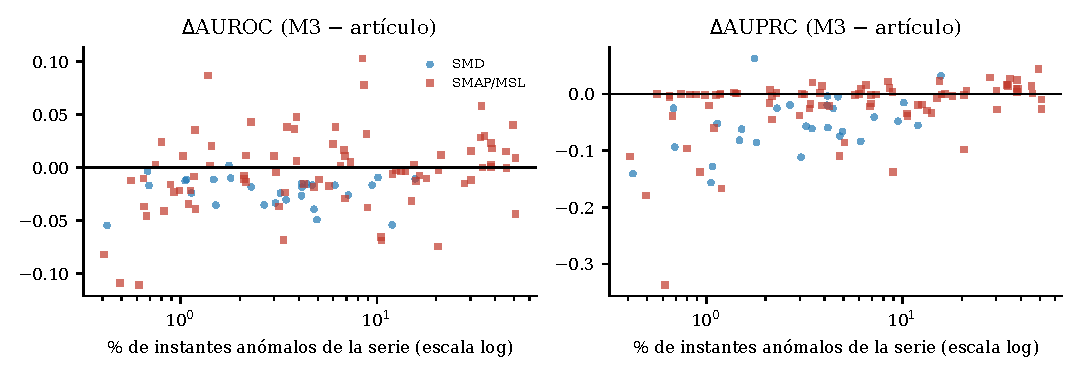
\includegraphics[width=.95\linewidth]{h6_tasa}
\caption{H6: ventaja de \MIII{} sobre el artículo (por serie, media de 5 semillas) frente a la tasa natural de
anomalías de la serie, en SMD y SMAP+MSL.}
\label{fig:h6}
\end{figure}
